\begin{figure}[htbp]
  \begin{tabular}{ccc}
    \begin{minipage}{0.33\hsize}
      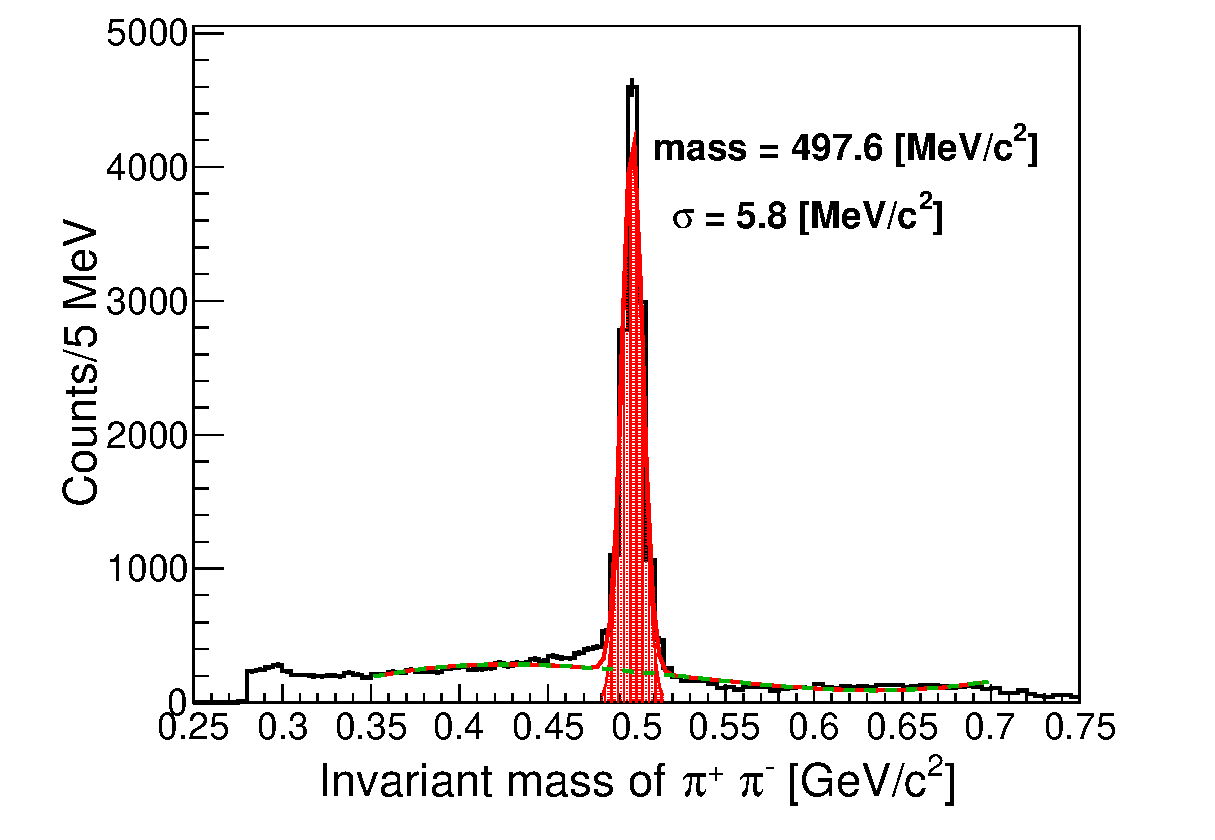
\includegraphics[width=4.5cm]{../pic/Run78/KN_ana_NC170_3sigma/IM_pipi_fitGauss.eps}
    \end{minipage}

    \begin{minipage}{0.33\hsize}
      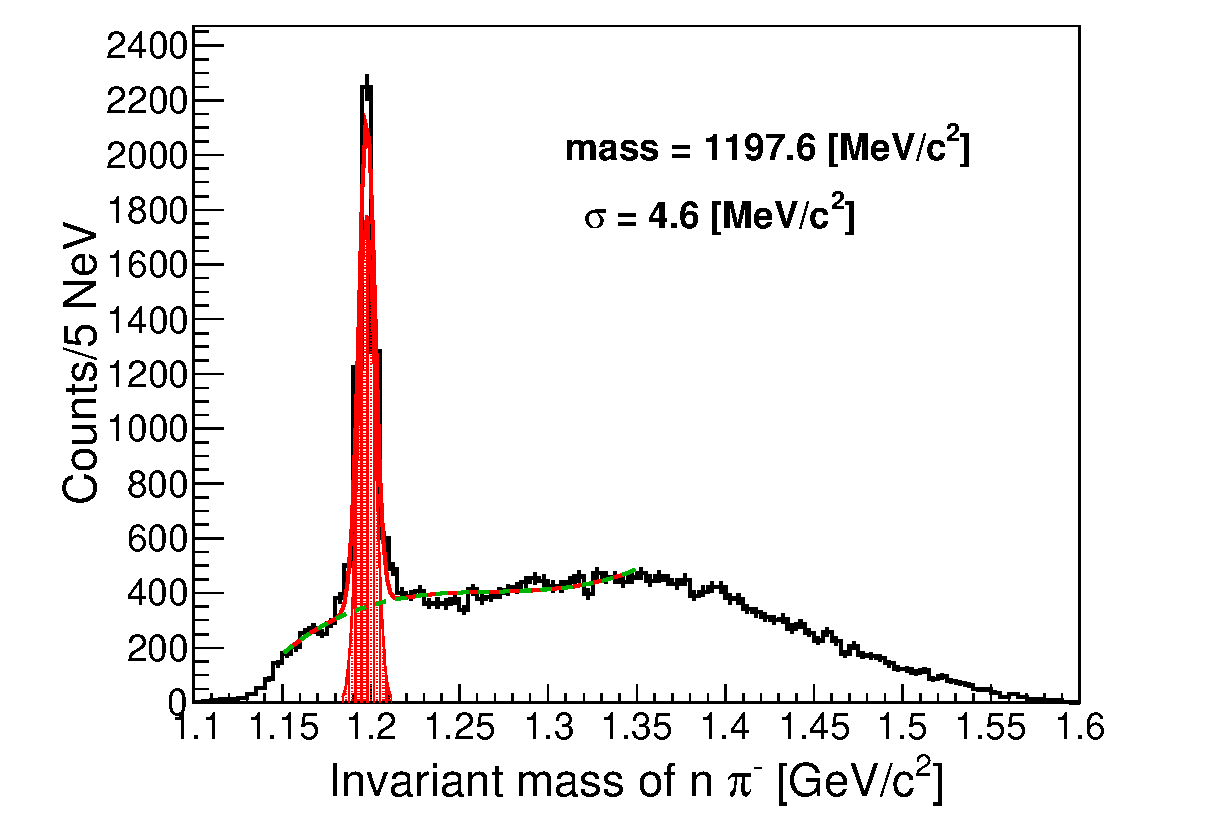
\includegraphics[width=4.5cm]{../pic/Run78/KN_ana_NC170_3sigma/IM_npim_fitGauss.eps}
    \end{minipage}

    \begin{minipage}{0.33\hsize}
      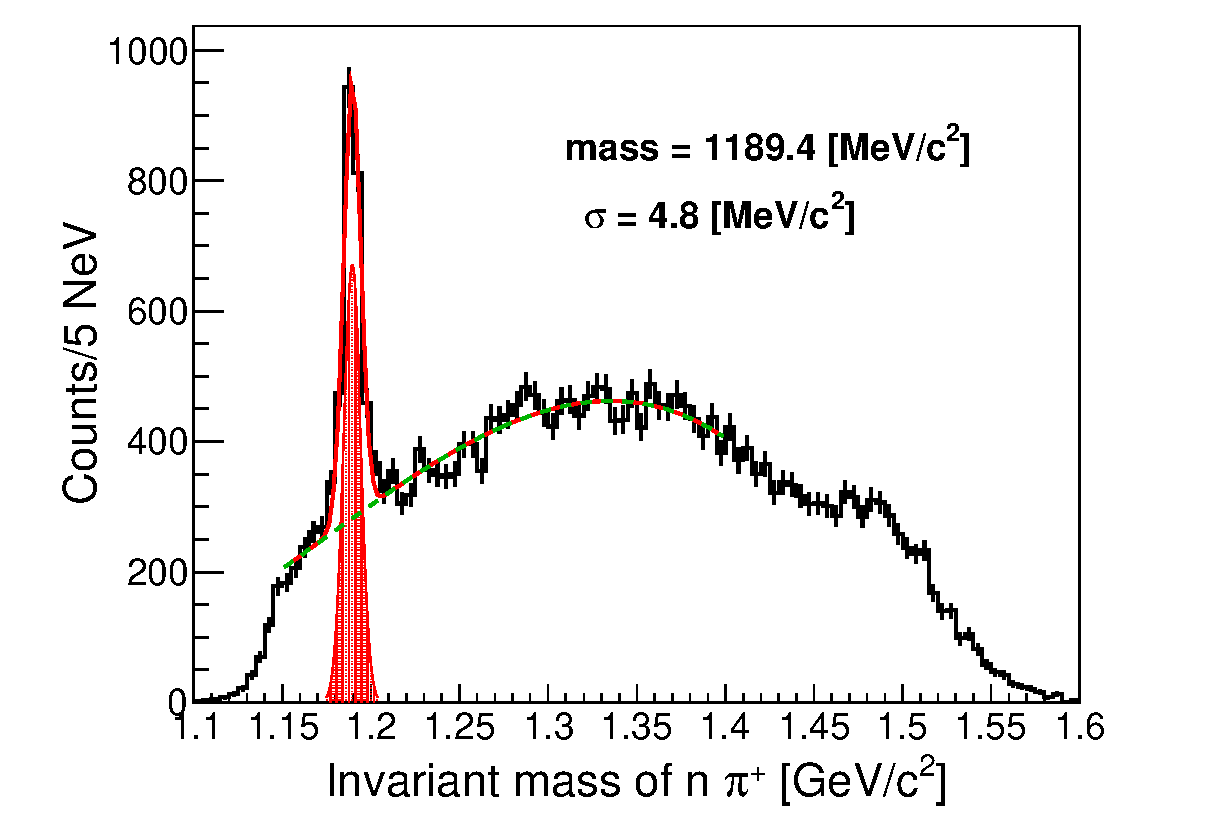
\includegraphics[width=4.5cm]{../pic/Run78/KN_ana_NC170_3sigma/IM_npip_fitGauss.eps}
    \end{minipage}
  \end{tabular}
  \caption{
    These figures show the invariant mass distributions of $\pi^+ \pi^-$,
    $n \pi^-$ and $n \pi^+$ in the $K d \rightarrow n \pi^+ \pi^- n$ event sample from left to right.
    The Gaussian functions and the selection regions for $K^0$ and $\Sigma^{\pm}_{forward}$ are indicated by red hatched area.
    The background third-order polynomial functions are shown as the green dashed lines.
  }
  \label{fig:npipin_IM_fitGauss}
\end{figure}
